\documentclass[11pt,a4paper]{article}
%%%%%%%%%%%%%%%%%%%%%%%%% Credit %%%%%%%%%%%%%%%%%%%%%%%%

% template ini dibuat oleh martin.manullang@if.itera.ac.id untuk dipergunakan oleh seluruh sivitas akademik itera.

%%%%%%%%%%%%%%%%%%%%%%%%% PACKAGE starts HERE %%%%%%%%%%%%%%%%%%%%%%%%
\usepackage{graphicx}
\usepackage{caption}
\usepackage{microtype}
\usepackage{lmodern}
\captionsetup[table]{name=Tabel}
\captionsetup[figure]{name=Gambar}
\usepackage{tabulary}
\usepackage{minted}
\usepackage{amsmath}
\usepackage{fancyhdr}
\usepackage{amssymb}
\usepackage{amsthm}
\usepackage{placeins}
\usepackage{amsfonts}
\usepackage{graphicx}
\usepackage[all]{xy}
\usepackage{tikz}
\usepackage{verbatim}
\usepackage[left=2cm,right=2cm,top=3cm,bottom=2.5cm]{geometry}
\usepackage{hyperref}
\hypersetup{
    colorlinks,
    linkcolor={red!50!black},
    citecolor={blue!50!black},
    urlcolor={blue!80!black}
}
\usepackage{caption}
\usepackage{subcaption}
\usepackage{multirow}
\usepackage{psfrag}
\usepackage[T1]{fontenc}
\usepackage[scaled]{beramono}
% Enable inserting code into the document
\usepackage{listings}
\usepackage{xcolor} 
% custom color & style for listing
\definecolor{codegreen}{rgb}{0,0.6,0}
\definecolor{codegray}{rgb}{0.5,0.5,0.5}
\definecolor{codepurple}{rgb}{0.58,0,0.82}
\definecolor{backcolour}{rgb}{0.95,0.95,0.92}
\definecolor{LightGray}{gray}{0.9}
\lstdefinestyle{mystyle}{
	backgroundcolor=\color{backcolour},   
	commentstyle=\color{green},
	keywordstyle=\color{codegreen},
	numberstyle=\tiny\color{codegray},
	stringstyle=\color{codepurple},
	basicstyle=\ttfamily\footnotesize,
	breakatwhitespace=false,         
	breaklines=true,                 
	captionpos=b,                    
	keepspaces=true,                 
	numbers=left,                    
	numbersep=5pt,                  
	showspaces=false,                
	showstringspaces=false,
	showtabs=false,                  
	tabsize=2
}
\lstset{style=mystyle}
\renewcommand{\lstlistingname}{Kode}
%%%%%%%%%%%%%%%%%%%%%%%%% PACKAGE ends HERE %%%%%%%%%%%%%%%%%%%%%%%%


%%%%%%%%%%%%%%%%%%%%%%%%% Data Diri %%%%%%%%%%%%%%%%%%%%%%%%
\newcommand{\student}{\textbf{Harisya Miranti (122140049)}}
\newcommand{\course}{\textbf{Sistem Teknologi Multimedia (IF25-40305)}}
\newcommand{\assignment}{\textbf{Worksheet 1: Setup Python Environment untuk Multimedia}}

%%%%%%%%%%%%%%%%%%% using theorem style %%%%%%%%%%%%%%%%%%%%
\newtheorem{thm}{Theorem}
\newtheorem{lem}[thm]{Lemma}
\newtheorem{defn}[thm]{Definition}
\newtheorem{exa}[thm]{Example}
\newtheorem{rem}[thm]{Remark}
\newtheorem{coro}[thm]{Corollary}
\newtheorem{quest}{Question}[section]
%%%%%%%%%%%%%%%%%%%%%%%%%%%%%%%%%%%%%%%%
\usepackage{lipsum}%% a garbage package you don't need except to create examples.
\usepackage{fancyhdr}
\pagestyle{fancy}
\lhead{Harisya Miranti (122140049)}
\rhead{ \thepage}
\cfoot{\textbf{Worksheet 1: Setup Python Environment untuk Multimedia}}
\renewcommand{\headrulewidth}{0.4pt}
\renewcommand{\footrulewidth}{0.4pt}

%%%%%%%%%%%%%%  Shortcut for usual set of numbers  %%%%%%%%%%%

\newcommand{\N}{\mathbb{N}}
\newcommand{\Z}{\mathbb{Z}}
\newcommand{\Q}{\mathbb{Q}}
\newcommand{\R}{\mathbb{R}}
\newcommand{\C}{\mathbb{C}}
\setlength\headheight{14pt}

%%%%%%%%%%%%%%%%%%%%%%%%%%%%%%%%%%%%%%%%%%%%%%%%%%%%%%%555
\begin{document}
\thispagestyle{empty}
\begin{center}
	\includegraphics[scale = 0.15]{Figure/ifitera-header.png}
	\vspace{0.1cm}
\end{center}
\noindent
\rule{17cm}{0.2cm}\\[0.3cm]
Nama: \student \hfill Tugas Ke: \assignment\\[0.1cm]
Mata Kuliah: \course \hfill Tanggal: \today\\
\rule{17cm}{0.05cm}
\vspace{0.1cm}



%%%%%%%%%%%%%%%%%%%%%%%%%%%%%%%%%%%%%%%%%%%%% BODY DOCUMENT %%%%%%%%%%%%%%%%%%%%%%%%%%%%%%%%%%%%%%%%%%%%%
\section{Tujuan Pembelajaran}
Setelah menyelesaikan worksheet ini, mahasiswa diharapkan mampu:
\begin{itemize}
    \item Memahami pentingnya manajemen environment Python untuk pengembangan multimedia
    \item Menginstall dan mengkonfigurasi Python environment menggunakan conda, venv, atau uv
    \item Menginstall library-library Python yang diperlukan untuk multimedia processing
    \item Memverifikasi instalasi dengan mengimpor dan menguji library multimedia
    \item Mendokumentasikan proses konfigurasi dan hasil pengujian dalam format \LaTeX
\end{itemize}

\section{Latar Belakang}
Python telah menjadi bahasa pemrograman yang sangat populer untuk multimedia processing karena memiliki ekosistem library yang sangat kaya. Namun, untuk dapat bekerja dengan multimedia secara efektif, kita perlu mengatur environment Python dengan benar dan menginstall library-library yang tepat.

Manajemen environment Python sangat penting untuk:
\begin{itemize}
    \item Menghindari konflik antar library (dependency conflict)
    \item Memastikan reproducibility dari project
    \item Memudahkan kolaborasi antar developer
    \item Memisahkan project yang berbeda dengan requirement yang berbeda
\end{itemize}

\section{Instruksi Tugas}

\subsection{Persiapan}
\textbf{Sebelum memulai, pastikan Anda telah:}
\begin{itemize}
    \item Menginstall Python 3.8 atau lebih baru di sistem Anda
    \item Memilih salah satu tool manajemen environment: \textbf{conda}, \textbf{venv}, atau \textbf{uv}
    \item Membuka terminal/command prompt
    \item Menyiapkan dokumen \LaTeX\ ini untuk dokumentasi
\end{itemize}

\subsection{Bagian 1: Membuat Environment Python}
Pilih \textbf{SALAH SATU} dari tiga opsi berikut dan ikuti langkah-langkahnya:

\subsubsection{Opsi 1: Menggunakan Conda (Direkomendasikan untuk pemula)}
Jalankan perintah berikut di terminal:

\begin{lstlisting}[language=bash, caption=Membuat environment dengan Conda]
# Membuat environment baru dengan nama 'multimedia'
conda create -n multimedia python=3.11

# Mengaktifkan environment
conda activate multimedia

# Verifikasi environment aktif
conda info --envs
\end{lstlisting}

\subsubsection{Opsi 2: Menggunakan venv (Built-in Python)}
\begin{lstlisting}[language=bash, caption=Membuat environment dengan venv]
# Membuat environment baru
python3 -m venv multimedia-env

# Mengaktifkan environment (Linux/Mac)
source multimedia-env/bin/activate

# Mengaktifkan environment (Windows)
# multimedia-env\Scripts\activate

# Verifikasi environment aktif
which python
\end{lstlisting}

\subsubsection{Opsi 3: Menggunakan uv (Modern dan cepat)}
\begin{lstlisting}[language=bash, caption=Membuat environment dengan uv]
# Install uv terlebih dahulu jika belum ada
# pip install uv

# Membuat environment baru
uv venv multimedia-uv

# Mengaktifkan environment (Linux/Mac)
source multimedia-uv/bin/activate

# Mengaktifkan environment (Windows)
# multimedia-uv\Scripts\activate

# Verifikasi environment aktif
which python
\end{lstlisting}

\textbf{Dokumentasikan di sini:}
\begin{itemize}
    \item Tool manajemen environment yang Anda pilih: \textbf{opsi 3 : uv}
    \item Screenshot atau copy-paste output dari perintah verifikasi environment
    \begin{center}
        \includegraphics[scale = 0.5]{Figure/verifikasiEnv.jpeg}
        \vspace{0.1cm}
    \end{center}
\end{itemize}

\subsection{Bagian 2: Instalasi Library Multimedia}
Setelah environment aktif, install library-library berikut:

\subsubsection{Library Audio Processing}
\begin{lstlisting}[language=bash, caption=Instalasi library audio]
# Untuk conda:
conda install -c conda-forge librosa soundfile scipy

# Untuk pip (venv/uv):
pip install librosa soundfile scipy
\end{lstlisting}

\subsubsection{Library Image Processing}
\begin{lstlisting}[language=bash, caption=Instalasi library image]
# Untuk conda:
conda install -c conda-forge opencv pillow scikit-image matplotlib

# Untuk pip (venv/uv):
pip install opencv-python pillow scikit-image matplotlib
\end{lstlisting}

\subsubsection{Library Video Processing}
\begin{lstlisting}[language=bash, caption=Instalasi library video]
# Untuk conda:
conda install -c conda-forge ffmpeg
pip install moviepy

# Untuk pip (venv/uv):
pip install moviepy
\end{lstlisting}

\subsubsection{Library General Purpose}
\begin{lstlisting}[language=bash, caption=Instalasi library umum]
# Untuk conda:
conda install numpy pandas jupyter

# Untuk pip (venv/uv):
pip install numpy pandas jupyter
\end{lstlisting}

\textbf{Dokumentasikan di sini:}
\begin{itemize}
    \item Perintah instalasi yang Anda gunakan
    \item Screenshot proses instalasi atau output sukses
    \item Daftar library yang berhasil diinstall dengan versinya
\end{itemize}

\subsection{Bagian 3: Verifikasi Instalasi}
Buat file Python sederhana untuk menguji semua library yang telah diinstall:
\begin{lstlisting}[language=bash, caption=Instalasi library image]
    # test_libs.py

print("=== TEST GENERAL LIBRARIES ===")
try:
    import numpy as np
    import pandas as pd
    print("NumPy version:", np.__version__)
    print("Pandas version:", pd.__version__)
except Exception as e:
    print("General libs error:", e)

print("\n=== TEST AUDIO LIBRARIES ===")
try:
    import librosa
    import soundfile as sf
    import scipy
    print("Librosa version:", librosa.__version__)
    print("SoundFile version:", sf.__version__)
    print("Scipy version:", scipy.__version__)
except Exception as e:
    print("Audio libs error:", e)

print("\n=== TEST IMAGE LIBRARIES ===")
try:
    import cv2
    from PIL import Image
    import skimage
    import matplotlib
    print("OpenCV version:", cv2.__version__)
    print("Pillow version:", Image.__version__)
    print("scikit-image version:", skimage.__version__)
    print("Matplotlib version:", matplotlib.__version__)
except Exception as e:
    print("Image libs error:", e)

print("\n=== TEST VIDEO LIBRARY ===")
try:
    import moviepy
    print("MoviePy version:", moviepy.__version__)
except Exception as e:
    print("Video lib error:", e)

print("\n Semua library berhasil di-import tanpa error!")
 scikit-image matplotlib
    \end{lstlisting}

\textbf{Jalankan script dan dokumentasikan hasilnya:}
\begin{center}
    \includegraphics[scale = 0.7]{Figure/verifikasiInstalasi.jpeg}
    \vspace{0.1cm}
\end{center}

\subsection{Bagian 4: Simple Test dengan Sample Code}
Buat dan jalankan contoh sederhana untuk setiap kategori multimedia:

\subsubsection{Test Audio Processing}
\begin{lstlisting}[language=Python, caption=Test audio processing sederhana]
import numpy as np
import matplotlib.pyplot as plt

# Generate simple sine wave
duration = 2  # seconds
sample_rate = 44100
frequency = 440  # A4 note

t = np.linspace(0, duration, int(sample_rate * duration))
audio_signal = np.sin(2 * np.pi * frequency * t)

# Plot waveform
plt.figure(figsize=(10, 4))
plt.plot(t[:1000], audio_signal[:1000])  # Plot first 1000 samples
plt.title('Sine Wave (440 Hz)')
plt.xlabel('Time (s)')
plt.ylabel('Amplitude')
plt.grid(True)
plt.savefig('sine_wave_test.png', dpi=150, bbox_inches='tight')
plt.show()

print(f"Generated {duration}s sine wave at {frequency}Hz")
print(f"Sample rate: {sample_rate}Hz")
print(f"Total samples: {len(audio_signal)}")
\end{lstlisting}

\subsubsection{Test Image Processing}
\begin{lstlisting}[language=Python, caption=Test image processing sederhana]
import numpy as np
import matplotlib.pyplot as plt
from PIL import Image

# Create a simple test image
width, height = 400, 300
image = np.zeros((height, width, 3), dtype=np.uint8)

# Add some patterns
image[:, :width//3, 0] = 255  # Red section
image[:, width//3:2*width//3, 1] = 255  # Green section
image[:, 2*width//3:, 2] = 255  # Blue section

# Add a white circle in the center
center_x, center_y = width//2, height//2
radius = 50
Y, X = np.ogrid[:height, :width]
mask = (X - center_x)**2 + (Y - center_y)**2 <= radius**2
image[mask] = [255, 255, 255]

# Display and save
plt.figure(figsize=(8, 6))
plt.imshow(image)
plt.title('Test Image with RGB Stripes and White Circle')
plt.axis('off')
plt.savefig('test_image.png', dpi=150, bbox_inches='tight')
plt.show()

print(f"Created test image: {width}x{height} pixels")
print(f"Image shape: {image.shape}")
print(f"Image dtype: {image.dtype}")
\end{lstlisting}

\textbf{Dokumentasikan hasil eksekusi:}
\begin{itemize}
    \item Screenshot output dari kedua script di atas
    \item Gambar yang dihasilkan (sine\_wave\_test.png dan test\_image.png)
    \item Error message jika ada dan cara mengatasinya
\end{itemize}

\section{Bagian Laporan}

\subsection{Output Verifikasi Instalasi}
\textbf{Copy-paste output lengkap dari script \texttt{test\_multimedia.py} di sini:}

\begin{lstlisting}[caption=Output verifikasi instalasi]
[PASTE OUTPUT DI SINI]
\end{lstlisting}

\subsection{Screenshot Hasil Test}
\textbf{Sisipkan screenshot atau gambar hasil dari:}
\begin{itemize}
    \item Terminal/command prompt yang menunjukkan environment aktif
    \begin{center}
        \includegraphics[scale = 0.7]{Figure/verifikasiInstalasi.jpeg}
        \vspace{0.1cm}
    \end{center}
    \item Output dari script test audio (sine wave plot)
    \begin{center}
        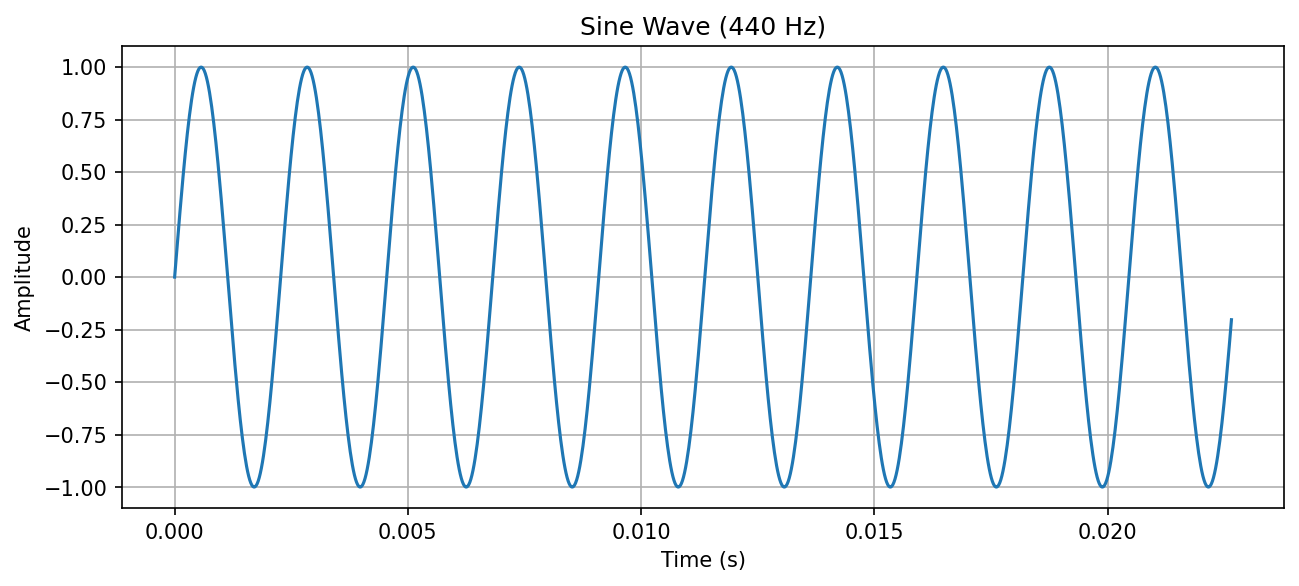
\includegraphics[scale = 0.7]{Figure/sine_wave_test.png}
        \vspace{0.1cm}
    \end{center}
    \item Output dari script test image (RGB stripes dengan circle)
    \begin{center}
        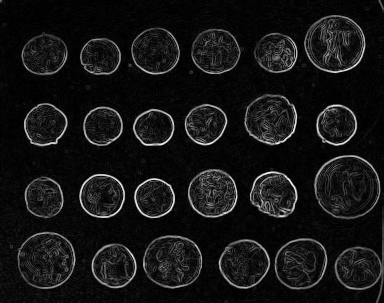
\includegraphics[scale = 0.7]{Figure/test_image.png}
        \vspace{0.1cm}
    \end{center}
\end{itemize}

\textit{Gunakan perintah \textbackslash\texttt{includegraphics} untuk menyisipkan gambar}

\subsection{Analisis dan Refleksi}
\textbf{Jawab pertanyaan berikut:}

\begin{enumerate}
    \item \textbf{Mengapa penting menggunakan environment terpisah untuk project multimedia?}
    
    \textit{karena environment penting untuk membantu menghindari terjadinya konflik antar project yang sudah dibuat, sehingga project dapat digunakan tanpa saling bentrok. }
    
    \item \textbf{Apa perbedaan utama antara conda, venv, dan uv? Mengapa Anda memilih tool yang Anda gunakan?}
    
    \textit{kalau conda lebih cocok untuk pengguna pemula sehingga lebih mudah untuk digunakan, kalau venv itu bawaan dari python jadi tidak perlu install tambahan, kalau uv lebih modern dan cepat. saya memilih uv karena uv kompatibel dengan ekosistem python dan praktis untuk project multimedia.}
    
    \item \textbf{Library mana yang paling sulit diinstall dan mengapa?}
    
    \textit{menurut pendapat saya yang paling sulit diinstall adalah conda, karena dilihat dari step yang banyak dan ukuran file yang besar.}
    
    \item \textbf{Bagaimana cara mengatasi masalah dependency conflict jika terjadi?}
    
    \textit{dengan cara selalu menggunakan virtual environment dan gunakan versi library yang paling cocok.}
    
    \item \textbf{Jelaskan fungsi dari masing-masing library yang berhasil Anda install!}
    
    \textit{library librosa, soundfile, dan scipy untuk mengolah file audio, opencv-python, pillow, scikit-image, matplotlib untuk mengolah file gambar, dan library moviepy berfungsi untuk mengolah file video. }
\end{enumerate}

\subsection{Troubleshooting}
\textbf{Dokumentasikan masalah yang Anda hadapi (jika ada) dan cara mengatasinya:}

\begin{itemize}
    \item \textbf{Masalah 1:} \textit{saat menginstall dependencies terjadi masalah konektivitas sehingga instal dependencies sering gagal dan berulang terus.}
    
    \textbf{Solusi:} \textit{menggunakan jaringan hotspot pribadi yang lebih kencang konektivitasnya}
    
    \item \textbf{Masalah 2:} \textit{salah memasukkan versi python saat ingin membuat virtual environment, yang harusnya versi 3.10, saya menggunakan versi 3.12.3}
    
    \textbf{Solusi:} \textit{membuat ulang virtual environment sesuai dengan versi python yang disarankan, yaitu versi 3.10}
\end{itemize}

\section{Export Environment untuk Reproduksi}
Sebagai langkah terakhir, export environment Anda agar dapat direproduksi:

\subsection{Untuk Conda}
\begin{lstlisting}[language=bash, caption=Export conda environment]
conda env export > environment.yml
\end{lstlisting}

\subsection{Untuk venv/uv}
\begin{lstlisting}[language=bash, caption=Export pip requirements]
pip freeze > requirements.txt
\end{lstlisting}

\textbf{Copy-paste isi file environment.yml atau requirements.txt di sini:}

\begin{lstlisting}[caption=Environment/Requirements file]
[anyio==4.10.0
argon2-cffi==25.1.0
argon2-cffi-bindings==25.1.0
arrow==1.3.0
asttokens==3.0.0
async-lru==2.0.5
attrs==25.3.0
audioread==3.0.1
babel==2.17.0
beautifulsoup4==4.13.5
bleach==6.2.0
certifi==2025.8.3
cffi==1.17.1
charset-normalizer==3.4.3
colorama==0.4.6
comm==0.2.3
contourpy==1.3.3
cycler==0.12.1
debugpy==1.8.16
decorator==5.2.1
defusedxml==0.7.1
executing==2.2.0
fastjsonschema==2.21.2
fonttools==4.59.2
fqdn==1.5.1
h11==0.16.0
httpcore==1.0.9
httpx==0.28.1
idna==3.10
imageio==2.37.0
imageio-ffmpeg==0.6.0
ipykernel==6.30.1
ipython==9.5.0
ipython-pygments-lexers==1.1.1
ipywidgets==8.1.7
isoduration==20.11.0
jedi==0.19.2
jinja2==3.1.6
joblib==1.5.2
json5==0.12.1
jsonpointer==3.0.0
jsonschema==4.25.1
jsonschema-specifications==2025.4.1
jupyter==1.1.1
jupyter-client==8.6.3
jupyter-console==6.6.3
jupyter-core==5.8.1
jupyter-events==0.12.0
jupyter-lsp==2.3.0
jupyter-server==2.17.0
jupyter-server-terminals==0.5.3
jupyterlab==4.4.6
jupyterlab-pygments==0.3.0
jupyterlab-server==2.27.3
jupyterlab-widgets==3.0.15
kiwisolver==1.4.9
lark==1.2.2
lazy-loader==0.4
librosa==0.11.0
llvmlite==0.44.0
markupsafe==3.0.2
matplotlib==3.10.5
matplotlib-inline==0.1.7
mistune==3.1.4
moviepy==2.2.1
msgpack==1.1.1
nbclient==0.10.2
nbconvert==7.16.6
nbformat==5.10.4
nest-asyncio==1.6.0
networkx==3.5
notebook==7.4.5
notebook-shim==0.2.4
numba==0.61.2
numpy==2.2.6
opencv-python==4.12.0.88
packaging==25.0
pandas==2.3.2
pandocfilters==1.5.1
parso==0.8.5
pillow==11.3.0
platformdirs==4.4.0
pooch==1.8.2
proglog==0.1.12
prometheus-client==0.22.1
prompt-toolkit==3.0.52
psutil==7.0.0
pure-eval==0.2.3
pycparser==2.22
pygments==2.19.2
pyparsing==3.2.3
python-dateutil==2.9.0.post0
python-dotenv==1.1.1
python-json-logger==3.3.0
pytz==2025.2
pywin32==311
pywinpty==3.0.0
pyyaml==6.0.2
pyzmq==27.0.2
referencing==0.36.2
requests==2.32.5
rfc3339-validator==0.1.4
rfc3986-validator==0.1.1
rfc3987-syntax==1.1.0
rpds-py==0.27.1
scikit-image==0.25.2
scikit-learn==1.7.1
scipy==1.16.1
send2trash==1.8.3
setuptools==80.9.0
six==1.17.0
sniffio==1.3.1
soundfile==0.13.1
soupsieve==2.8
soxr==0.5.0.post1
stack-data==0.6.3
terminado==0.18.1
threadpoolctl==3.6.0
tifffile==2025.8.28
tinycss2==1.4.0
tornado==6.5.2
tqdm==4.67.1
traitlets==5.14.3
types-python-dateutil==2.9.0.20250822
typing-extensions==4.15.0
tzdata==2025.2
uri-template==1.3.0
urllib3==2.5.0
wcwidth==0.2.13
webcolors==24.11.1
webencodings==0.5.1
websocket-client==1.8.0
widgetsnbextension==4.0.14
]
\end{lstlisting}

\section{Kesimpulan}
\textbf{Tuliskan kesimpulan Anda mengenai:}
\begin{itemize}
    \item Pengalaman setup Python environment untuk multimedia
    \item Persiapan untuk project multimedia selanjutnya
    \item Saran untuk mahasiswa lain yang akan melakukan setup serupa
\end{itemize}

\textit{pengetahuan baru tentang instalansi environment python yang akan digunakan dalam pembelajaran multimedia, dan cara menangani trouble yang dihadapi saat proses penginstalan yang dibantu oleh AI dan teman yang sudah berhasil menginstal duluan. Persiapan untuk project multimedia selanjutnya adalah mulai mencari tahu terkait library yang akan digunakan seperti library audio, video, dan gambar. saran untuk teman mahasiswa lainnya adalah jangan ragu untuk menanyakan kendala yang dihadapi ke teman yang sudah tahu dan berhasil melakukan setup.}

\section{Referensi}
Sertakan referensi yang Anda gunakan selama proses setup dan troubleshooting.

\newpage
\bibliographystyle{IEEEtran}
\bibliography{Referensi}
chatGPT: https://chatgpt.com/share/68b1b8df-81f8-8013-8f68-e76e33994c77
rekan sejawat: Elma Nurul fatika
\end{document}